\scanpage{56}

\figure{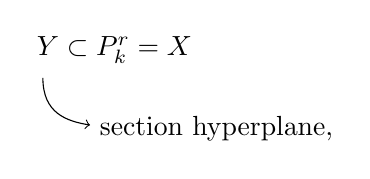
\begin{tikzpicture}[x=1cm,y=1cm]
\node[anchor=west] at (0,1) {$Y\subset P^r_k=X$};
\node[anchor=west] at (.8,0) {section hyperplane,};
\draw[->] (.2,.65) .. controls (.2,.2) and (.5,.1) .. (.8,.05);
\end{tikzpicture}}
$U$ voisinage de $Y$, $Z=X-U$
\inserted{ens. \unsure{fermé|fini} fini}

$F$ cohérent sur $X$

a) Condition pour que $H^i(U,F(-m))=0$ pour $m$ grand?

\unsure{a')|d)} Condition pour que
$\unsure{\coprod_m|\bigoplus_m}H^i(U,F(m))$ de type fini sur $S$

b) Condition pour que $H^i(U,F(m))=0$ pour $m$ grand

($i>0$ donné)

\unsure{c)} Condition pour que
\[
H^i(U,F)\longrightarrow H^i(\hat X,\hat F)
\]
soit un isomorphisme?

\figure{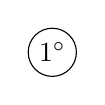
\begin{tikzpicture}\node[draw,circle,inner sep=2pt] {$1^\circ$};\end{tikzpicture}}
Considérons la suite exacte
(où $E^d=\underline{\operatorname{Ext}}^d_{O_X}(F,\omega_X)$)

\diagram{\begin{tikzcd}[column sep=small,row sep=large]
H^i_Z(X,F(\unsure{-m}))\arrow[r,"\alpha_i"]&
H^i(X,F(\unsure{-m}))\arrow[r]&
H^i(U,F(\unsure{-m}))\arrow[r]&
H^{i+1}_Z(X,F(\unsure{-m}))\arrow[r,dash,"\alpha_{i+1}"]&
H^{i+1}(X,F(-m))\\
\prod_{z\in Z}\bigl(E^{r-i}(m)\bigr)^\wedge_z&
\Gamma E^{r-i}(m)\arrow[l]&&
\prod_{z\in Z}\bigl(E^{r-i-1}(m)\bigr)^\wedge_z&
\Gamma E^{r-i-1}(m)\arrow[l]
\end{tikzcd}}

Conditions équivalentes

\diagram{\begin{tikzcd}[row sep=large]
\alpha_i\ \text{surjectif pour }m\text{ grand}
\quad\deleted{\text{\unsure{pour tout $m$}}}
\arrow[d,Leftrightarrow]\arrow[dd,bend right=65]\quad\\
z\in Z\ \Rightarrow\ z\text{ isolé dans }(\operatorname{supp}E^{r-i}\cup\{z\})
\arrow[d,Leftrightarrow]\\
H^{i-1}(X,F(-m))\longrightarrow H^{i-1}(U,F(-m))
\quad\text{\uline{surjectif} pour }m\text{ grand}
\end{tikzcd}}

\margin{\unsure{*}}
\diagram{\begin{tikzcd}[row sep=large]
\alpha_i\ \text{injectif pour }m\text{ grand},\quad i\leq n\quad\Longleftrightarrow
\arrow[d,Leftrightarrow]\\
\exists\text{ voisinage ouvert }V\text{ de }Z,\text{ tel que }F
\text{ soit de profondeur }>n\text{ sur }U\cap V
\arrow[d,Leftrightarrow]\\
H^i(X,F(-m))\mathbin{-}H^i(U,F(-m))\quad
\text{surjectif pour }m\text{ grand},\ i<n
\end{tikzcd}}

\figure{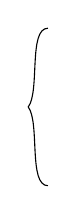
\begin{tikzpicture}[x=1cm,y=1cm]
\draw (.25,2) .. controls (0,2) and (.15,1.2) .. (0,1)
 .. controls (.15,.8) and (0,0) .. (.25,0);
\end{tikzpicture}}

\margin{55}
